%   Copyright (C) 2021 Greenweaves Software Limited
%
%   This program is free software: you can redistribute it and/or
%   modify it under the terms of the GNU Lesser General Public
%   License as published by the Free Software Foundation; either
%   version 2.1 of the License, or (at your option) any later version.
%
%  This program is distributed in the hope that it will be useful,
%  but WITHOUT ANY WARRANTY; without even the implied warranty of
%  MERCHANTABILITY or FITNESS FOR A PARTICULAR PURPOSE.  See the
%  GNU  Lesser General Public License for more details
%
%  You should have received a copy of the GNU Lesser General Public License
%  along with this program.  If not, see <https://www.gnu.org/licenses/>.
%
%  To contact me, Simon Crase, email simon@greenweaves.nz


\documentclass[]{article}
\usepackage[acronym,toc,nonumberlist]{glossaries}
\usepackage{glossaries-extra}
\usepackage{url}
\usepackage{float}
\usepackage{caption}
\usepackage{subcaption}
\usepackage{graphicx}
\usepackage{amsmath}
\usepackage{amssymb}
\usepackage{tocloft}
\usepackage[document]{ragged2e}
\usepackage{longtable}
\graphicspath{{figs/}}
\makeglossaries
\loadglsentries{glossary-entries}
\pdfpxdimen=1in
\divide\pdfpxdimen by 300

%opening
\title{Human Protein Atlas - Single Cell Classification\\Notes}
\author{Simon Crase}

\begin{document}

\maketitle


\begin{abstract}
My notes on the Human Protein Atlas - Single Cell Classification project.
\end{abstract}
\tableofcontents
\listoftables
\listoffigures
\section{The Task}

\begin{quotation}
	The labels are the organelles/structures in which the proteins are located. So you are correct in assuming that the labels only apply to the cells where green is present (as the green is the protein).
	
	If there are 4 cells and 3 have green staining and the image-level labels are Mitochondria, and Nucleoplasm.
	
	Cell 1:
	- Green looks to be in the Mitochondria. Therefore, the cell level is Mitochondria.
	
	Cell 2:
	- Green looks to be in the Nucleoplasm. Therefore, the cell level is Nucleoplasm.
	
	Cell 3:
	- Green looks to be in the Nucleoplasm and Mitochondria. Therefore, the cell level label is Nucleoplasm and Mitochondria
	
	Cell 4:
	- No green or green is not present in any organelle. Therefore, the cell level label is Negative. \cite{schettler2021}
\end{quotation}


\begin{longtable}{|r|p{ 0.9\textwidth}|}
	\caption{Labels}\\  \hline
	Code&Description\\ \hline
	\endfirsthead
\hline	Code&Description\\ \hline
	\endhead
 0&\Gls{nucleoplasm}: \glsdesc{nucleoplasm} \\ \hline
 1&\Gls{nuclear_membrane}: \glsdesc{nuclear_membrane}\\ \hline
 2&\Glspl{nucleolus}: \glsdesc{nucleolus}\\ \hline
 3&\Gls{nucleolus_fibrillar_center}: \glsdesc{nucleolus_fibrillar_center}\\ \hline
 4&\Gls{nuclear_speckles}: \glsdesc{nuclear_speckles}\\ \hline
 5&\Gls{nuclear_bodies}: \glsdesc{nuclear_bodies}\\ \hline
 6&\Gls{endoplasmic_reticulum}: \glsdesc{endoplasmic_reticulum}\\ \hline
 7&\Gls{golgi_apparatus}: \glsdesc{golgi_apparatus}\\ \hline
 8&\Gls{intermediate_filament}: \glsdesc{intermediate_filament}\\ \hline
 9&\Gls{actin} filaments: \glsdesc{actin}\\\hline
 10&\Gls{microtubules}: \glsdesc{microtubules}\\\hline
 11&\Gls{mitotic_spindle}: \glsdesc{mitotic_spindle}\\\hline
 12&\Gls{centrosome}: \glsdesc{centrosome}\\\hline
 13&\Gls{plasma_membrane}: \glsdesc{plasma_membrane}\\\hline
 14&\Glspl{mitochondrion}: \glsdesc{mitochondrion}\\\hline
 15&\Gls{aggresome}: \glsdesc{aggresome}\\\hline
 16&\Gls{cytosol}: \glsdesc{cytosol}\\\hline
 17&\Glspl{vesicle} and \gls{punctate} cytosolic patterns : \glsdesc{vesicle}\\\hline
 18&Negative \\ \hline
\end{longtable}


Metric for evaluation--\gls{mAP}.

\section{Segmentation}

\begin{itemize}
	\item Usually in biological images, cells are crowded and cell borders are hard to tell (especially in tissue), so a common protocol is to segment the nuclei first, and use them as seeds to segment the cells--\cite{liao2021ground}.
	\item My first na\"ive version of Watershed wasn't successful, but check out \cite{najman1994watershed}.
	\item Try Otsu's method \cite{otsu1979threshold} combined with exploration of 8-connected neighbourhood.
	 \cite{win2018comparative}
	\item \cite{jo2021puzzle}
\end{itemize}

\begin{figure}
	\caption[Nucleoplasm: protein appears to overlap nucleus closely]{Nucleoplasm: protein appears to overlap nucleus closely}
	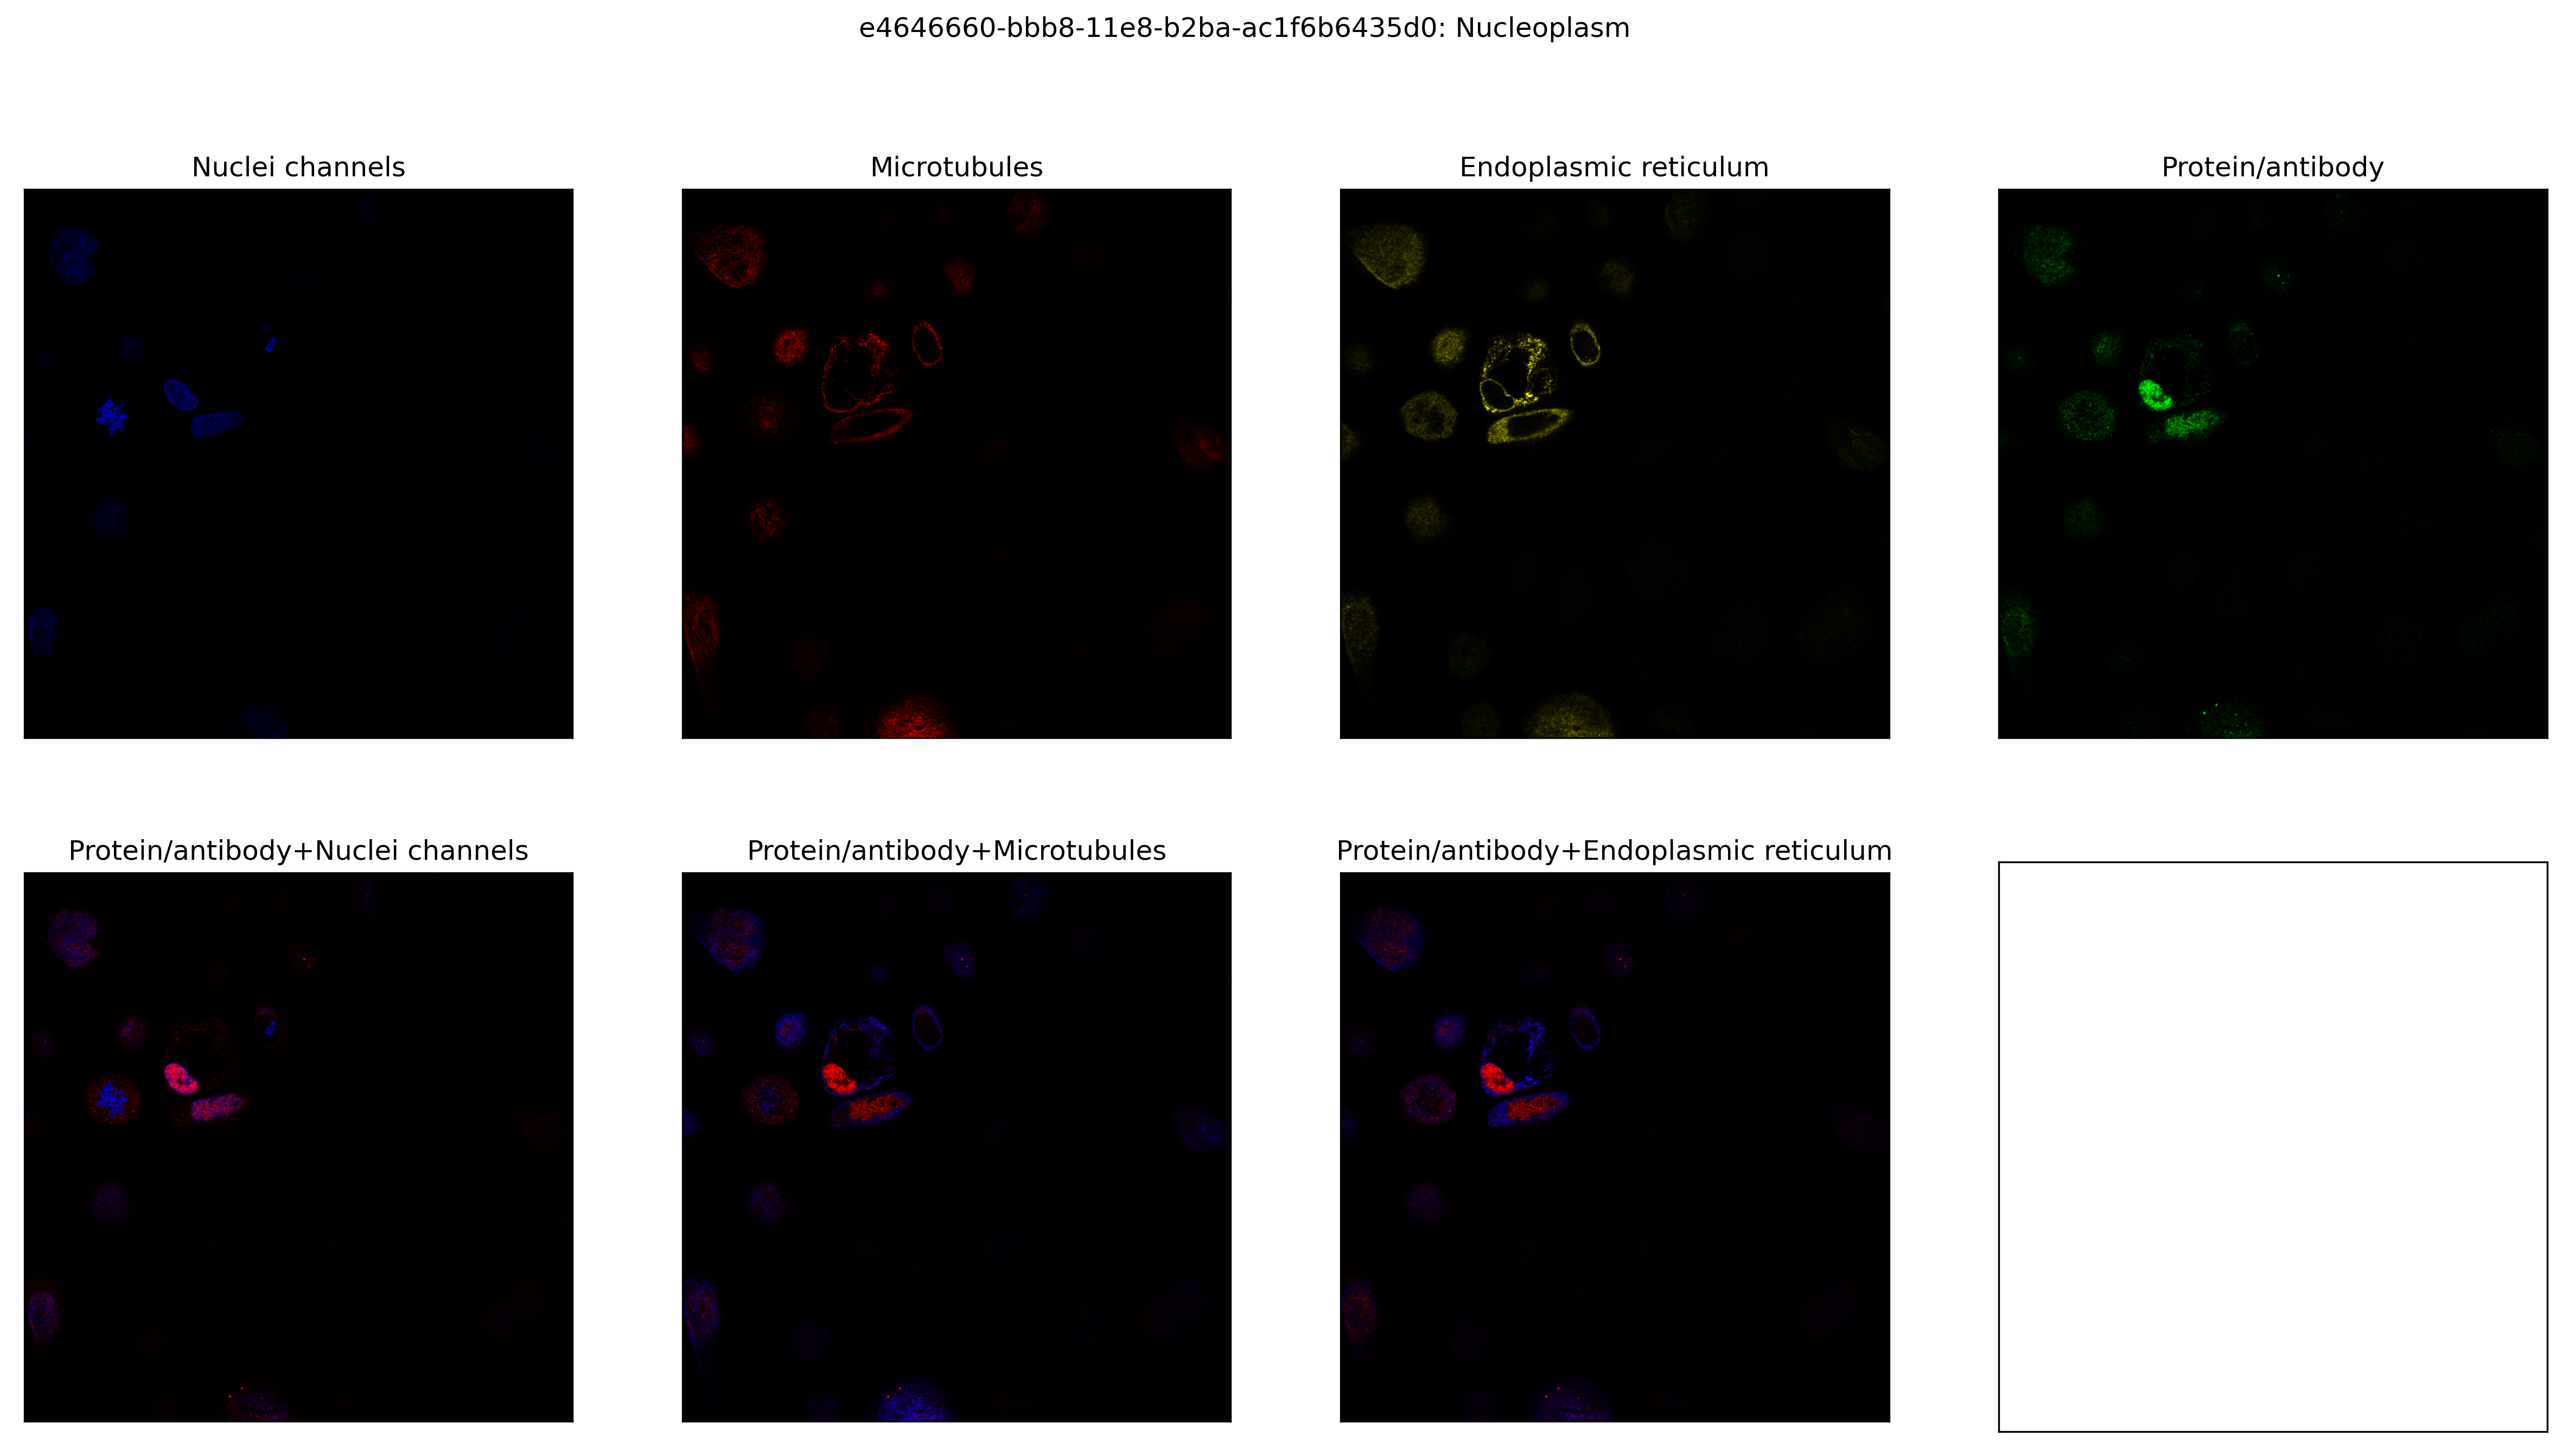
\includegraphics[width=\textwidth]{e4646660-bbb8-11e8-b2ba-ac1f6b6435d0}
	\includegraphics[width=\textwidth]{a45378f8-bbb4-11e8-b2ba-ac1f6b6435d0}
\end{figure}

\begin{figure}
	\caption[Nucleoplasm with other labels]{Nucleoplasm with other labels}
	\includegraphics[width=\textwidth]{dc12ada8-bba1-11e8-b2b9-ac1f6b6435d0}
	\includegraphics[width=\textwidth]{8793a49c-bb99-11e8-b2b9-ac1f6b6435d0}
\end{figure}

\begin{figure}
	\caption[Nuclear Membrane: protein appears to halo nucleus]{Nucleoplasm: protein appears to halo nucleus}
	\includegraphics[width=\textwidth]{ec0badb6-bbb7-11e8-b2ba-ac1f6b6435d0}
	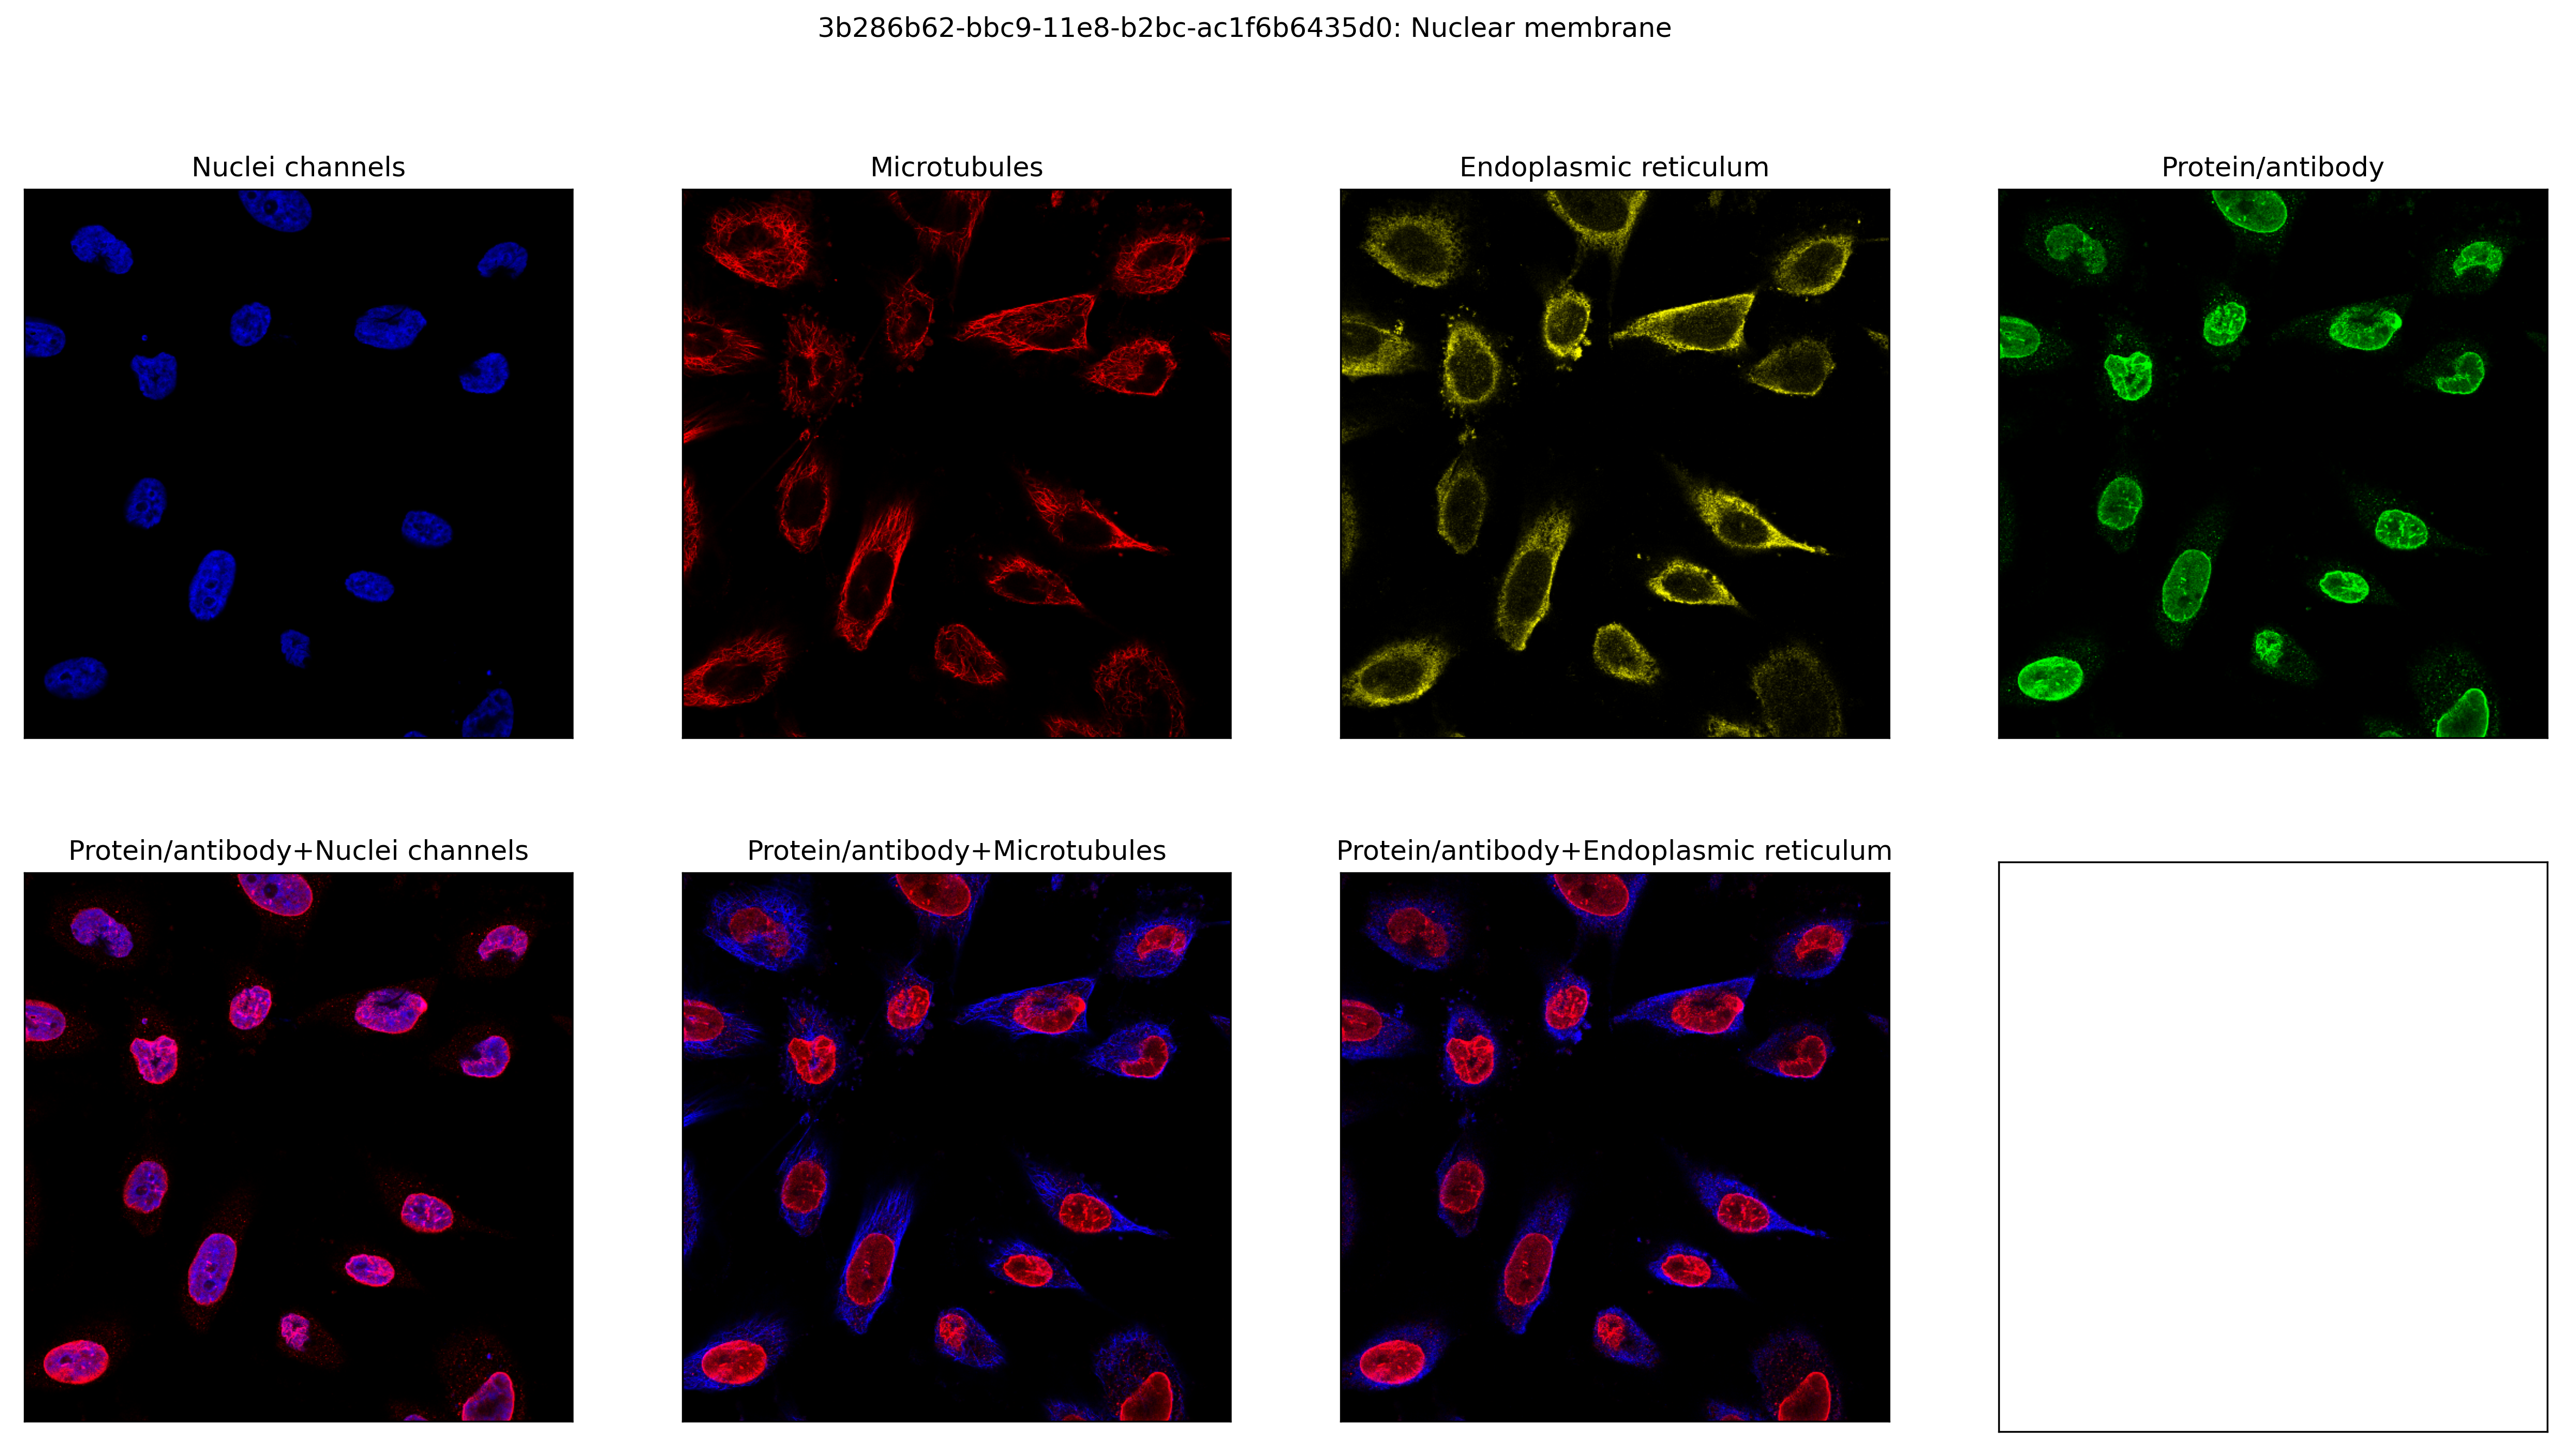
\includegraphics[width=\textwidth]{3b286b62-bbc9-11e8-b2bc-ac1f6b6435d0}
\end{figure}

\begin{figure}
	\caption{Nucleoli}
	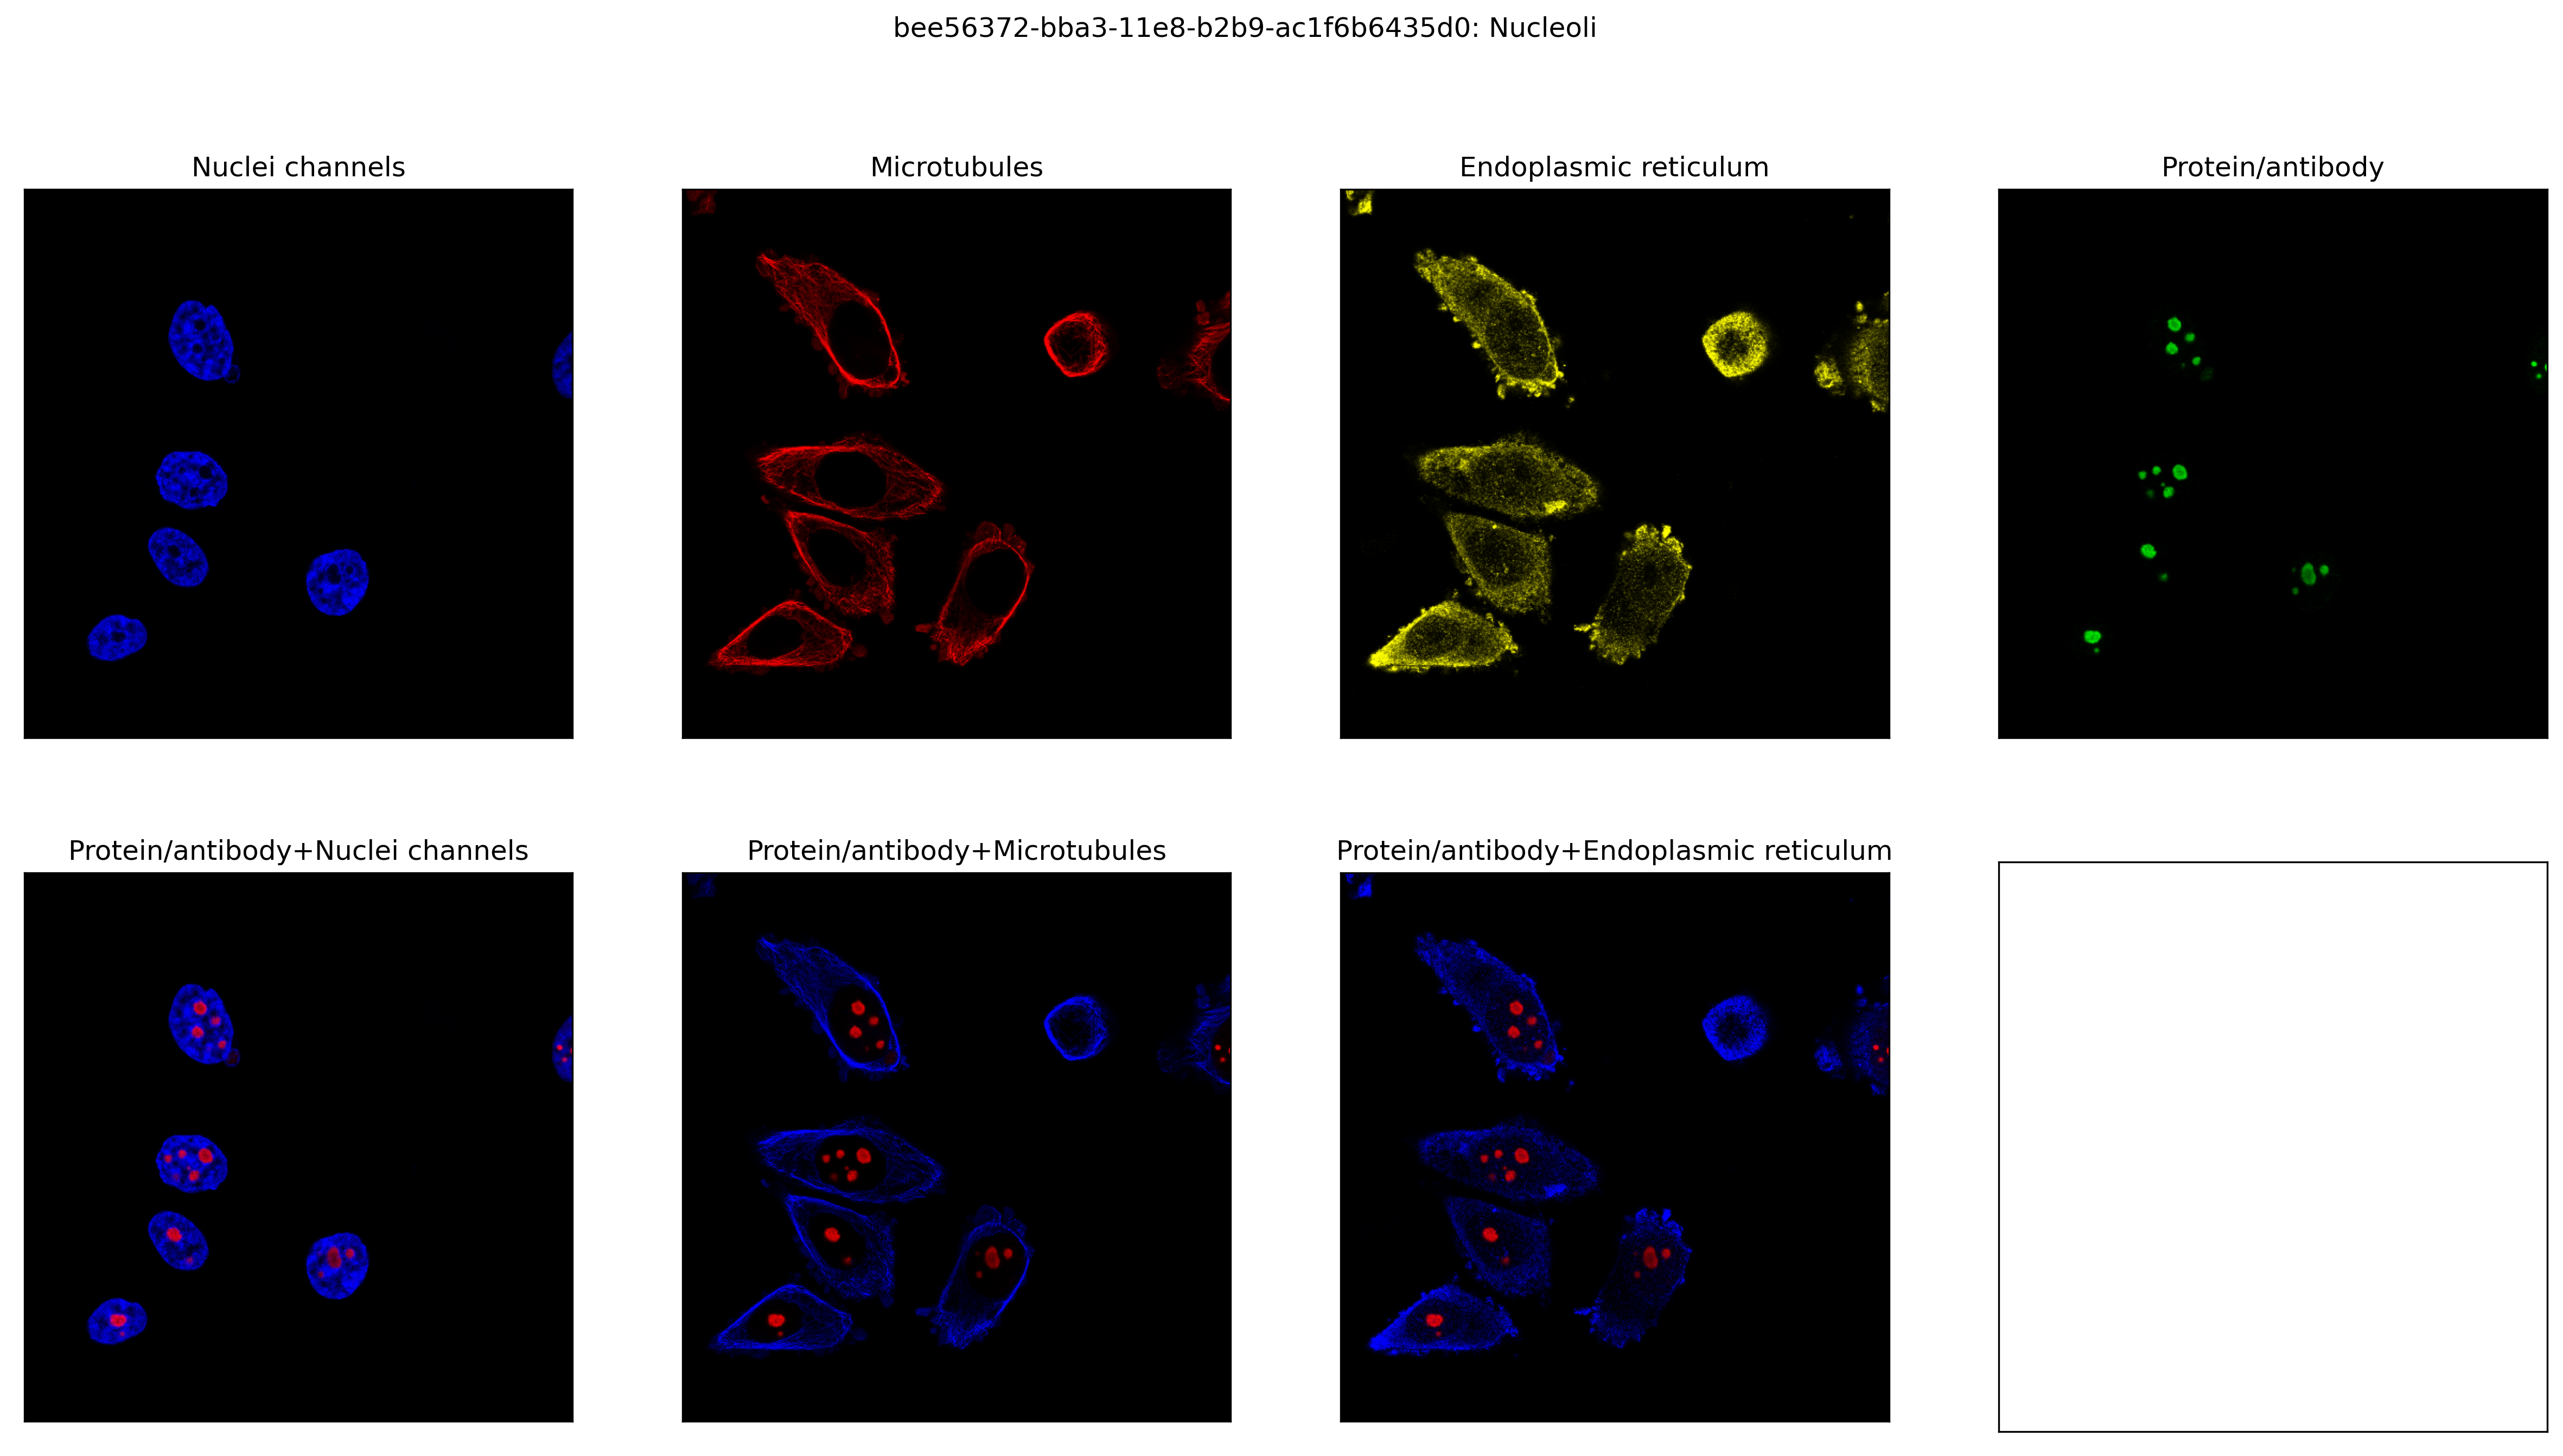
\includegraphics[width=\textwidth]{bee56372-bba3-11e8-b2b9-ac1f6b6435d0}
	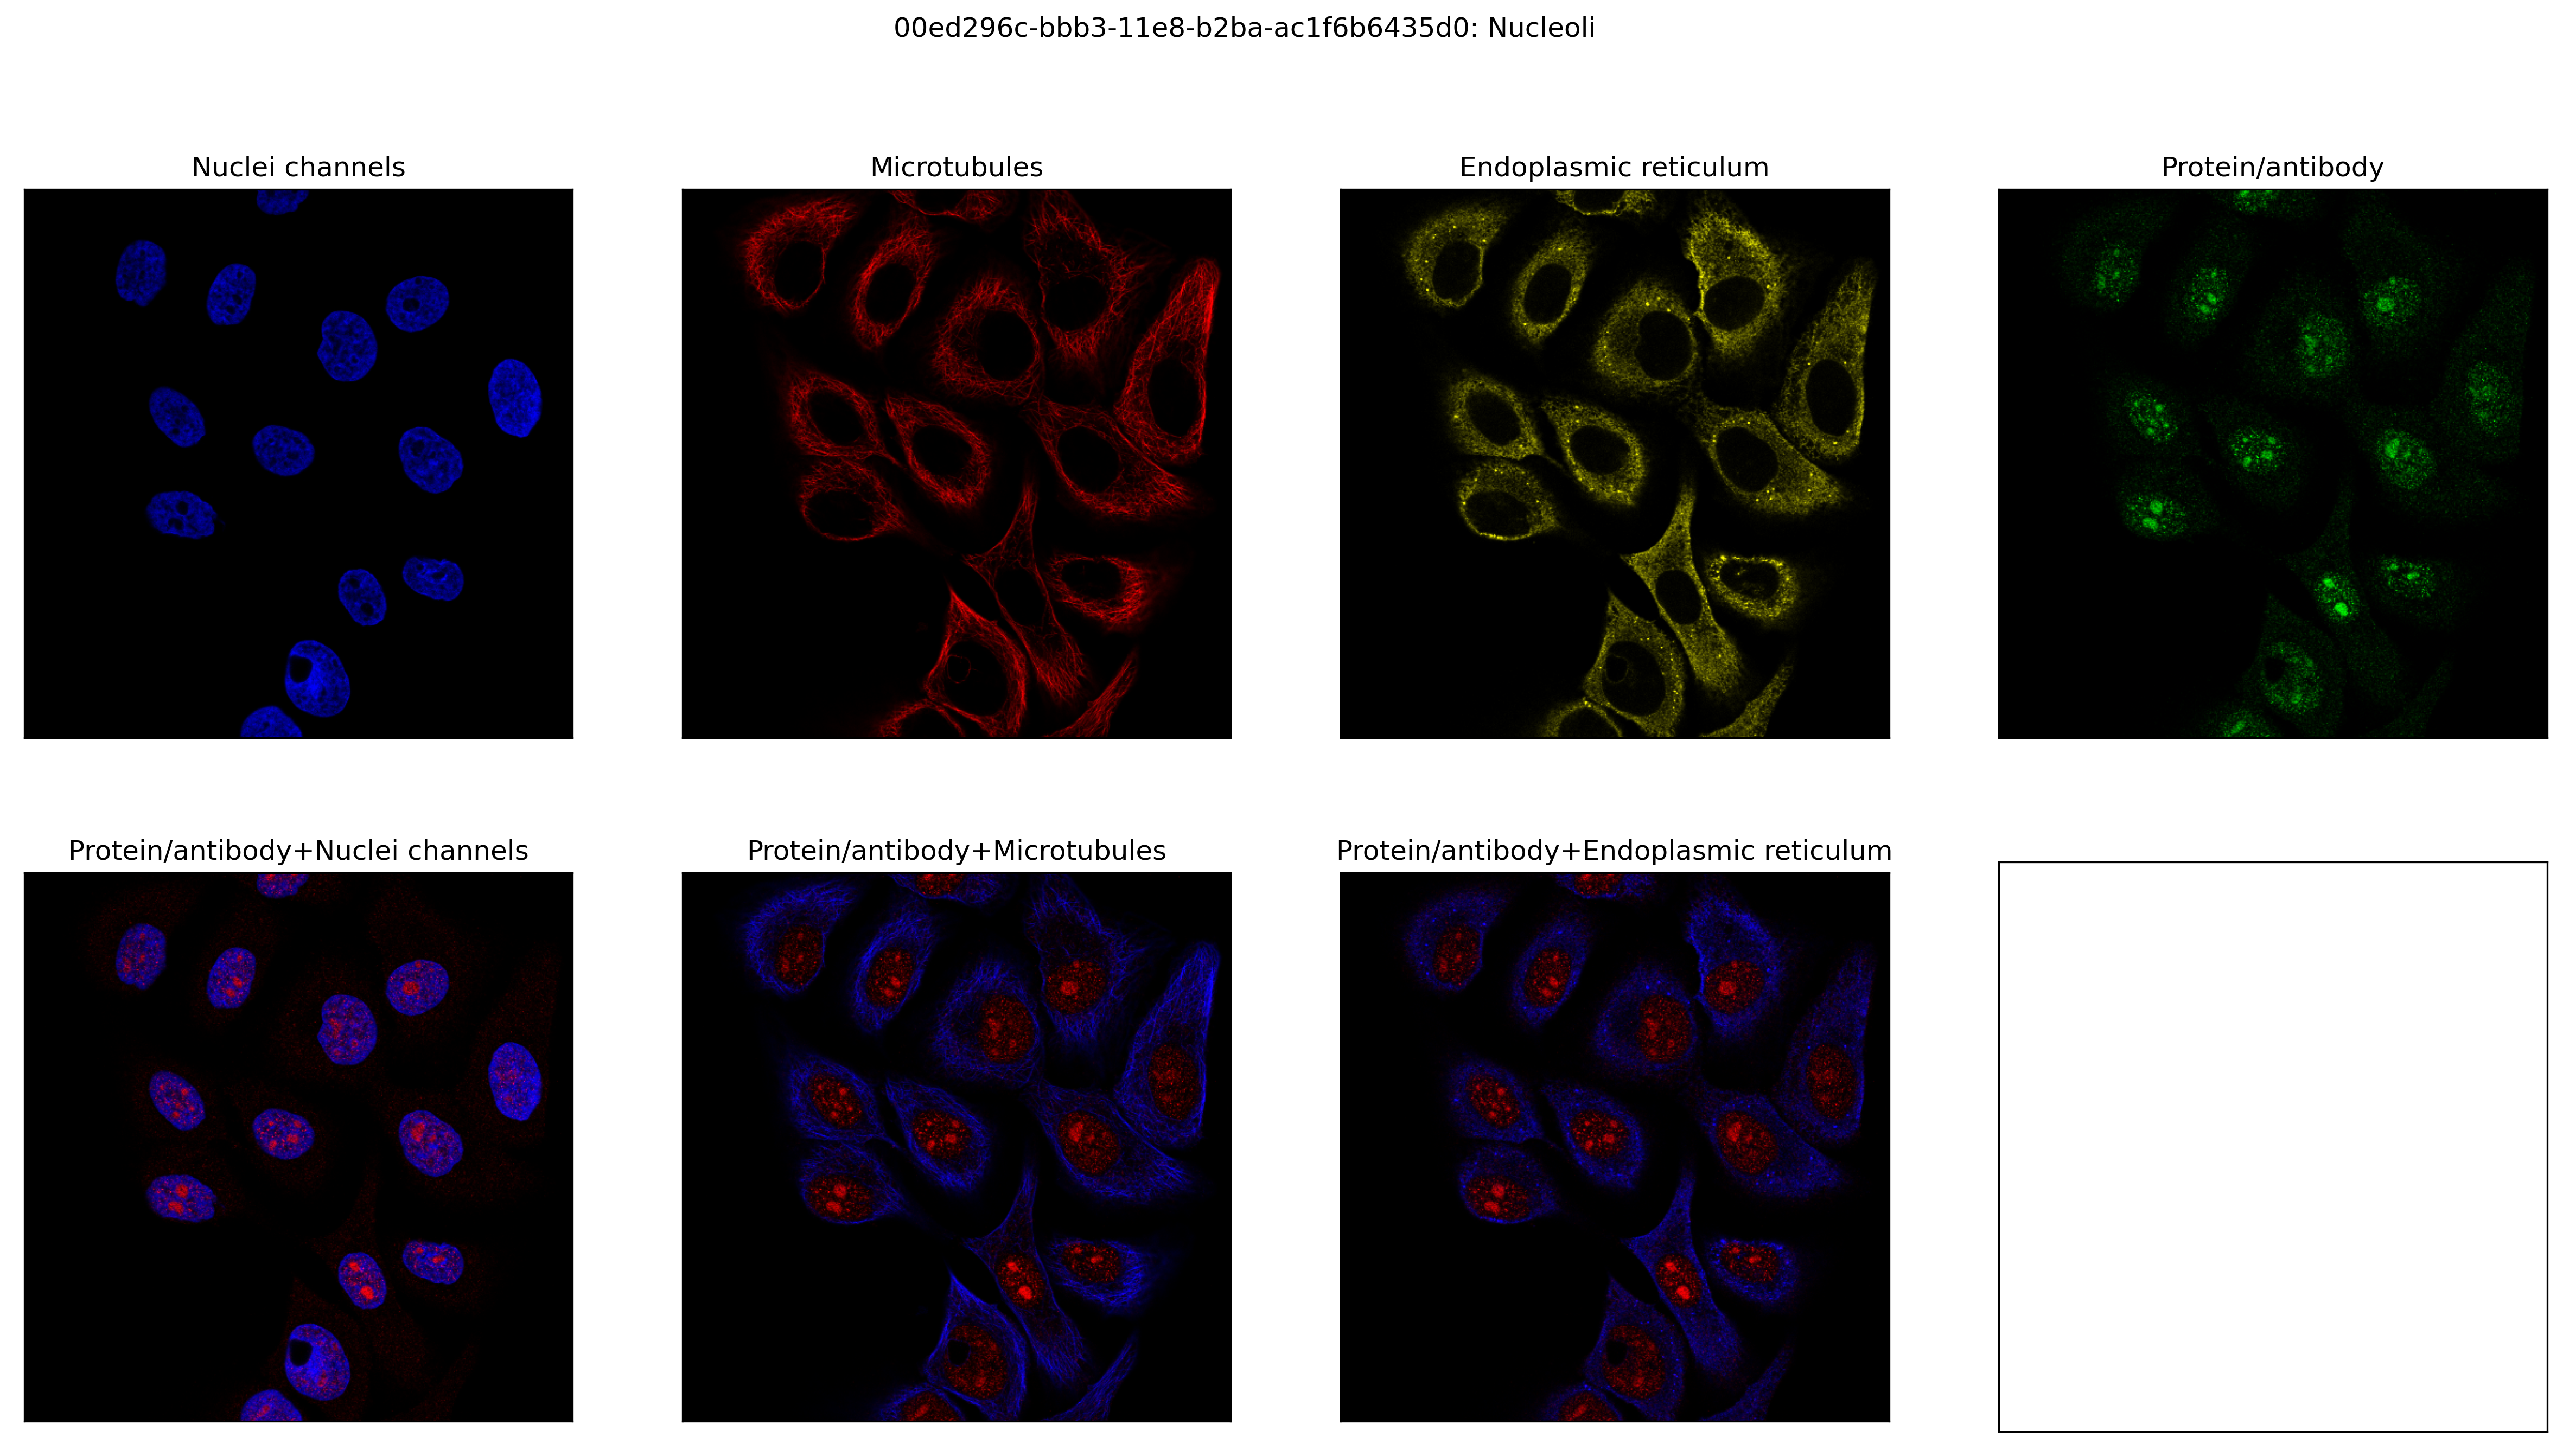
\includegraphics[width=\textwidth]{00ed296c-bbb3-11e8-b2ba-ac1f6b6435d0}
\end{figure}

\begin{figure}
	\caption{Nucleolus fibrillar center}
	\includegraphics[width=\textwidth]{5b30d3c6-bbc5-11e8-b2bc-ac1f6b6435d0}
	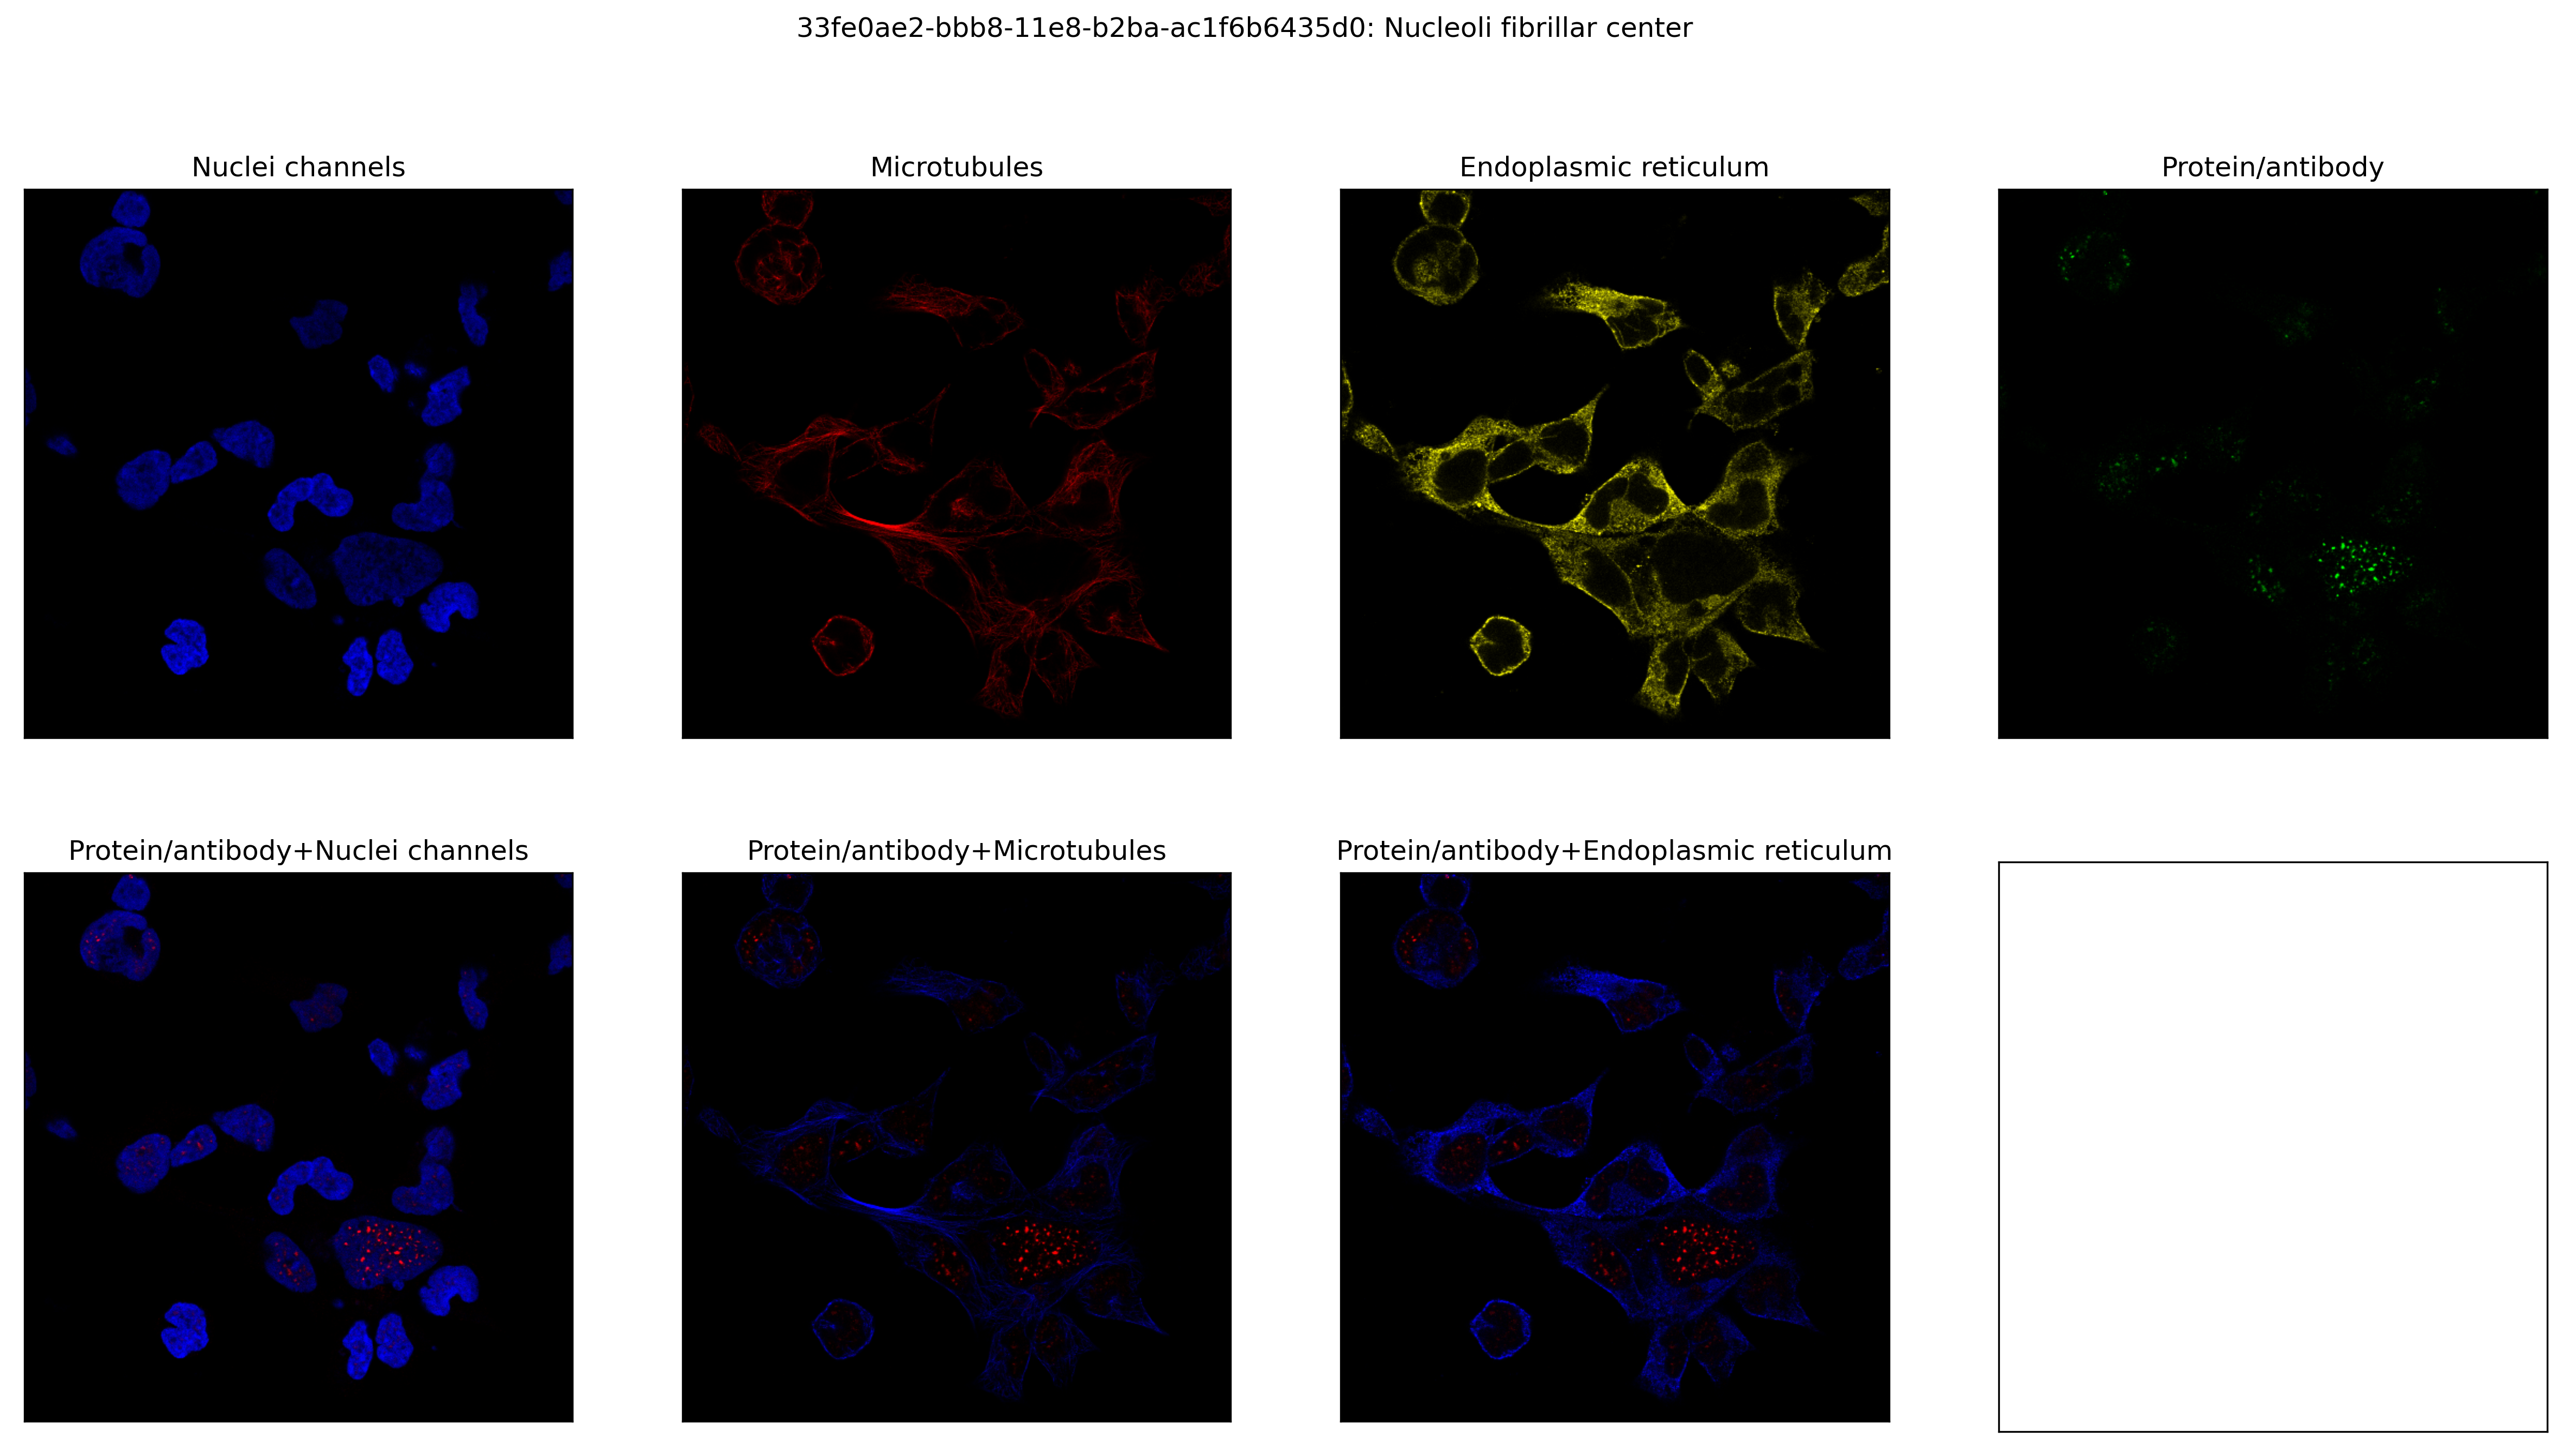
\includegraphics[width=\textwidth]{33fe0ae2-bbb8-11e8-b2ba-ac1f6b6435d0}
\end{figure}

\begin{figure}
	\caption{Microtubules}
	\includegraphics[width=\textwidth]{d18a5b1a-bbba-11e8-b2ba-ac1f6b6435d0}
	\includegraphics[width=\textwidth]{0cd92bf2-bbab-11e8-b2ba-ac1f6b6435d0}
\end{figure}

\clearpage


\printacronyms
\printglossary

\bibliographystyle{unsrt}
\addcontentsline{toc}{section}{Bibliography}
\bibliography{hpa-scc}
\end{document}
